\documentclass{standalone}
\usepackage{tikz}
\usepackage{pgfplots}
\usepackage{pgf-spectra}

\def \plotwidth {510.0pt}
\def \tth{3.16227766017}

\definecolor{color1}{RGB}{202,0,32}
\definecolor{color2}{RGB}{244,165,130}
\definecolor{color3}{RGB}{146,197,222}
\definecolor{color4}{RGB}{5,113,176}

\newcommand{\styleone}{densely dotted}
\newcommand{\styletwo}{densely dashed}
\newcommand{\stylethree}{dashdotted}
\newcommand{\stylefour}{solid}
\newcommand{\stylefive}{loosely dashed}

\def\linethickness{0.8pt}

\begin{document}
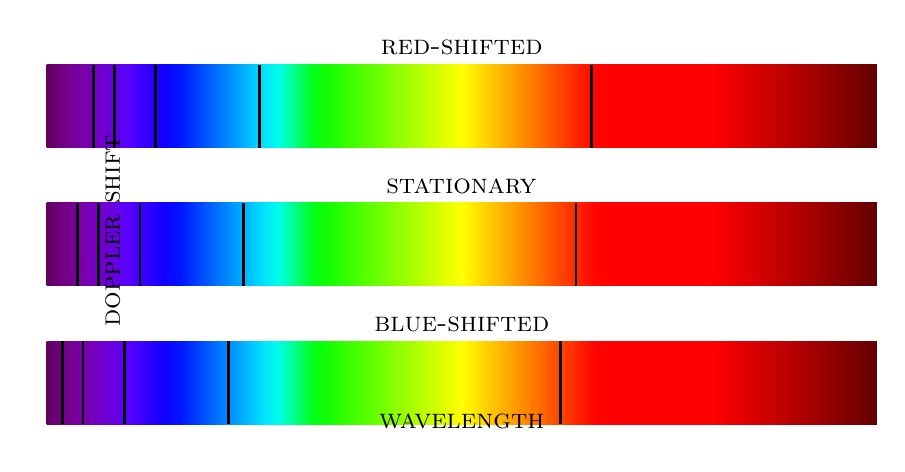
\begin{tikzpicture}
\begin{axis}[
	width=\textwidth, height=185pt,
	axis line style={draw=none},
	xmin=380, xmax=780,
	ymin=0, ymax=1.5,
	xlabel={\textsc{wavelength}},
	ylabel={\textsc{doppler shift}},
	x label style={at={(axis description cs: 0.5, 0.05)}, rotate=0, anchor=north},
	y label style={at={(axis description cs: 0.1, 0.5)}, rotate=0, anchor=south},
	xtick={},
	xticklabels={},
	minor xtick={},
	xtick style={draw=none},
	ytick={},
	yticklabels={},
	minor ytick={},
	ytick style={draw=none},
	legend columns=1,
	legend style={draw=none, at={(axis cs: 0, 0)}, anchor=south west,},
	axis on top,
]
	\put(0, 99.5pt) {\pgfspectra[lines={402.5, 412.5, 432.5, 482.5, 642.5}, absorption, height=30pt, width=300pt]};
	\node[anchor=south] at (150pt, 130pt) {\textsc{red-shifted}};
	\put(0, 49.5pt) {\pgfspectra[lines={395, 405, 425, 475, 635}, absorption, height=30pt, width=300pt]};
	\node[anchor=south] at (150pt, 80pt) {\textsc{stationary}};
	\put(0, -0.5pt) {\pgfspectra[lines={387.5, 397.5, 417.5, 467.5, 627.5}, absorption, height=30pt, width=300pt]};
	\node[anchor=south] at (150pt, 30pt) {\textsc{blue-shifted}};
\end{axis}
\end{tikzpicture}
\end{document}